\section{Phylogenetics and phylodynamics}
\label{sec:phylo}

\subsection{Phylogenetic trees}

In evolutionary biology, a \defn{phylogeny}, or \defn{phylogenetic tree}, is a
graphical representation of the the evolutionary relationships among a group of
organisms or species (generally, \defn{taxa})~\autocite{haeckel1866generelle}.
The \defn{tips} of a phylogeny, that is, the nodes without any descendants,
correspond to \defn{extant}, or observed, taxa, while the \defn{internal nodes}
correspond to their common ancestors. The edges or \defn{branches} of the
phylogeny connect ancestors to their descendants. Phylogenies may have a
\defn{root}, which is a node with no descendants distinguished as the most
recent common ancestor of all the extant
taxa~\autocite{harding1971probabilities}. When such a root exists, the tree is
referred to as being \defn{rooted}; otherwise, it is \defn{unrooted}. The
structural arrangement of nodes and edges in the tree is referred to as its
\defn{topology}~\autocite{cavalli1967phylogenetic}. 

The branches of the tree may have associated lengths, representing either
evolutionary distance or calendar time between ancestors and their descendants.
The term ``evolutionary distance'' is used here imprecisely to mean any sort of
quantitative measure of evolution, such as the number of differences between
the DNA sequences of an ancestor its descendant, or the difference in average
body mass or height. A phylogeny with branch lengths in calendar time units is
often referred to as \defn{time-scaled}. In a time-scaled phylogeny, the
internal nodes can be mapped onto a timeline by using the tips of the tree,
which usually correspond to the present day, as a reference
point~\autocite{nee1992tempo}. The corresponding points on the timeline are
called \defn{branching times}, and the rate of their accumulation is referred
to as the \defn{branching rate}. Rooted trees whose tips are all the same
distance from the root are called \defn{ultrametric}
trees~\autocite{buneman1974note}. These concepts are illustrated in
\cref{fig:speciestree}.

\begin{figure}[ht]
  \centering
  \includegraphics{speciestree.pdf}
  \caption[Illustration of a rooted, ultrametric, time-scaled phylogeny]
    {Illustration of a rooted, ultrametric, time-scaled phylogeny. The tips of
      the tree, which represent extant taxa, are placed at the present day on
      the time axis. Internal nodes, representing extinct common ancestors to
      the extant taxa, fall in the past. The topology of the tree indicates
      that cats and dogs are the most closely related pair of species, whereas
      fish is most distantly related to any other node in the tree.}
  \label{fig:speciestree}
\end{figure}

\subsection{Transmission trees}

In epidemiology, a \defn{transmission tree} is a graphical representation of an
epidemic's progress through a population. Like phylogenies, transmission trees
have tips, nodes, edges, and branch lengths. However, rather than recording an
evolutionary process (speciation), they record an epidemiological process
(transmission). The tips of a transmission tree represent infected hosts, while
internal nodes correspond to transmissions from one host to another.
Transmission trees generally have branch lengths in units of calendar time,
with branching times indicating times of transmission. The root of a
transmission tree corresponds to the initially infected patient who introduced
the epidemic into the network, also known as the \defn{index case}. The
internal nodes may be labelled with the donor of the transmission pair, if this
is known. The tips of the tree, rather than being fixed at the present day, are
placed at the time at which the individual was removed from the epidemic, such
as by death, recovery, isolation, behaviour change, or migration. Consequently,
the transmission tree may not be ultrametric, but may have tips located at
varying distances from the root. Such trees are said to have
\defn{heterochronous} taxa~\autocite{drummond2003measurably}, in contrast to
the \defn{isochronous} taxa found in most phylogenies of macro-organisms. A
transmission tree is illustrated in \cref{fig:contactnet} (right). 

Due to the internal nodes, each infected individual in an epidemic may appear
in the transmission tree more than once. This is different from the
transmission \emph{network}, in which each infected individual appears exactly
once, and edges are in one-to-one correspondence with
transmissions~\autocite{welch2011statistical, keeling2005networks}.
Transmission networks are discussed further in \cref{sec:contactnet}, and the
distinction between the two objects is illustrated in \cref{fig:contactnet}.
However, since transmission networks generally have no cycles (unless
re-infection occurs), they are trees in the graph theoretical sense, and hence
are sometimes also referred to as transmission
trees~\autocite[\eg][]{kenah2015algorithms}. In this work, we reserve the term
``transmission tree'' for the objects depicted on the right side of
\cref{fig:contactnet}, following~\autocite[\eg][]{stadler2013uncovering}. The
term ``transmission network'' is taken to mean the subgraph of the contact
network along which transmissions occurred,
following~\autocite{welch2011statistical, keeling2005networks}.

\begin{figure}
    \centering
    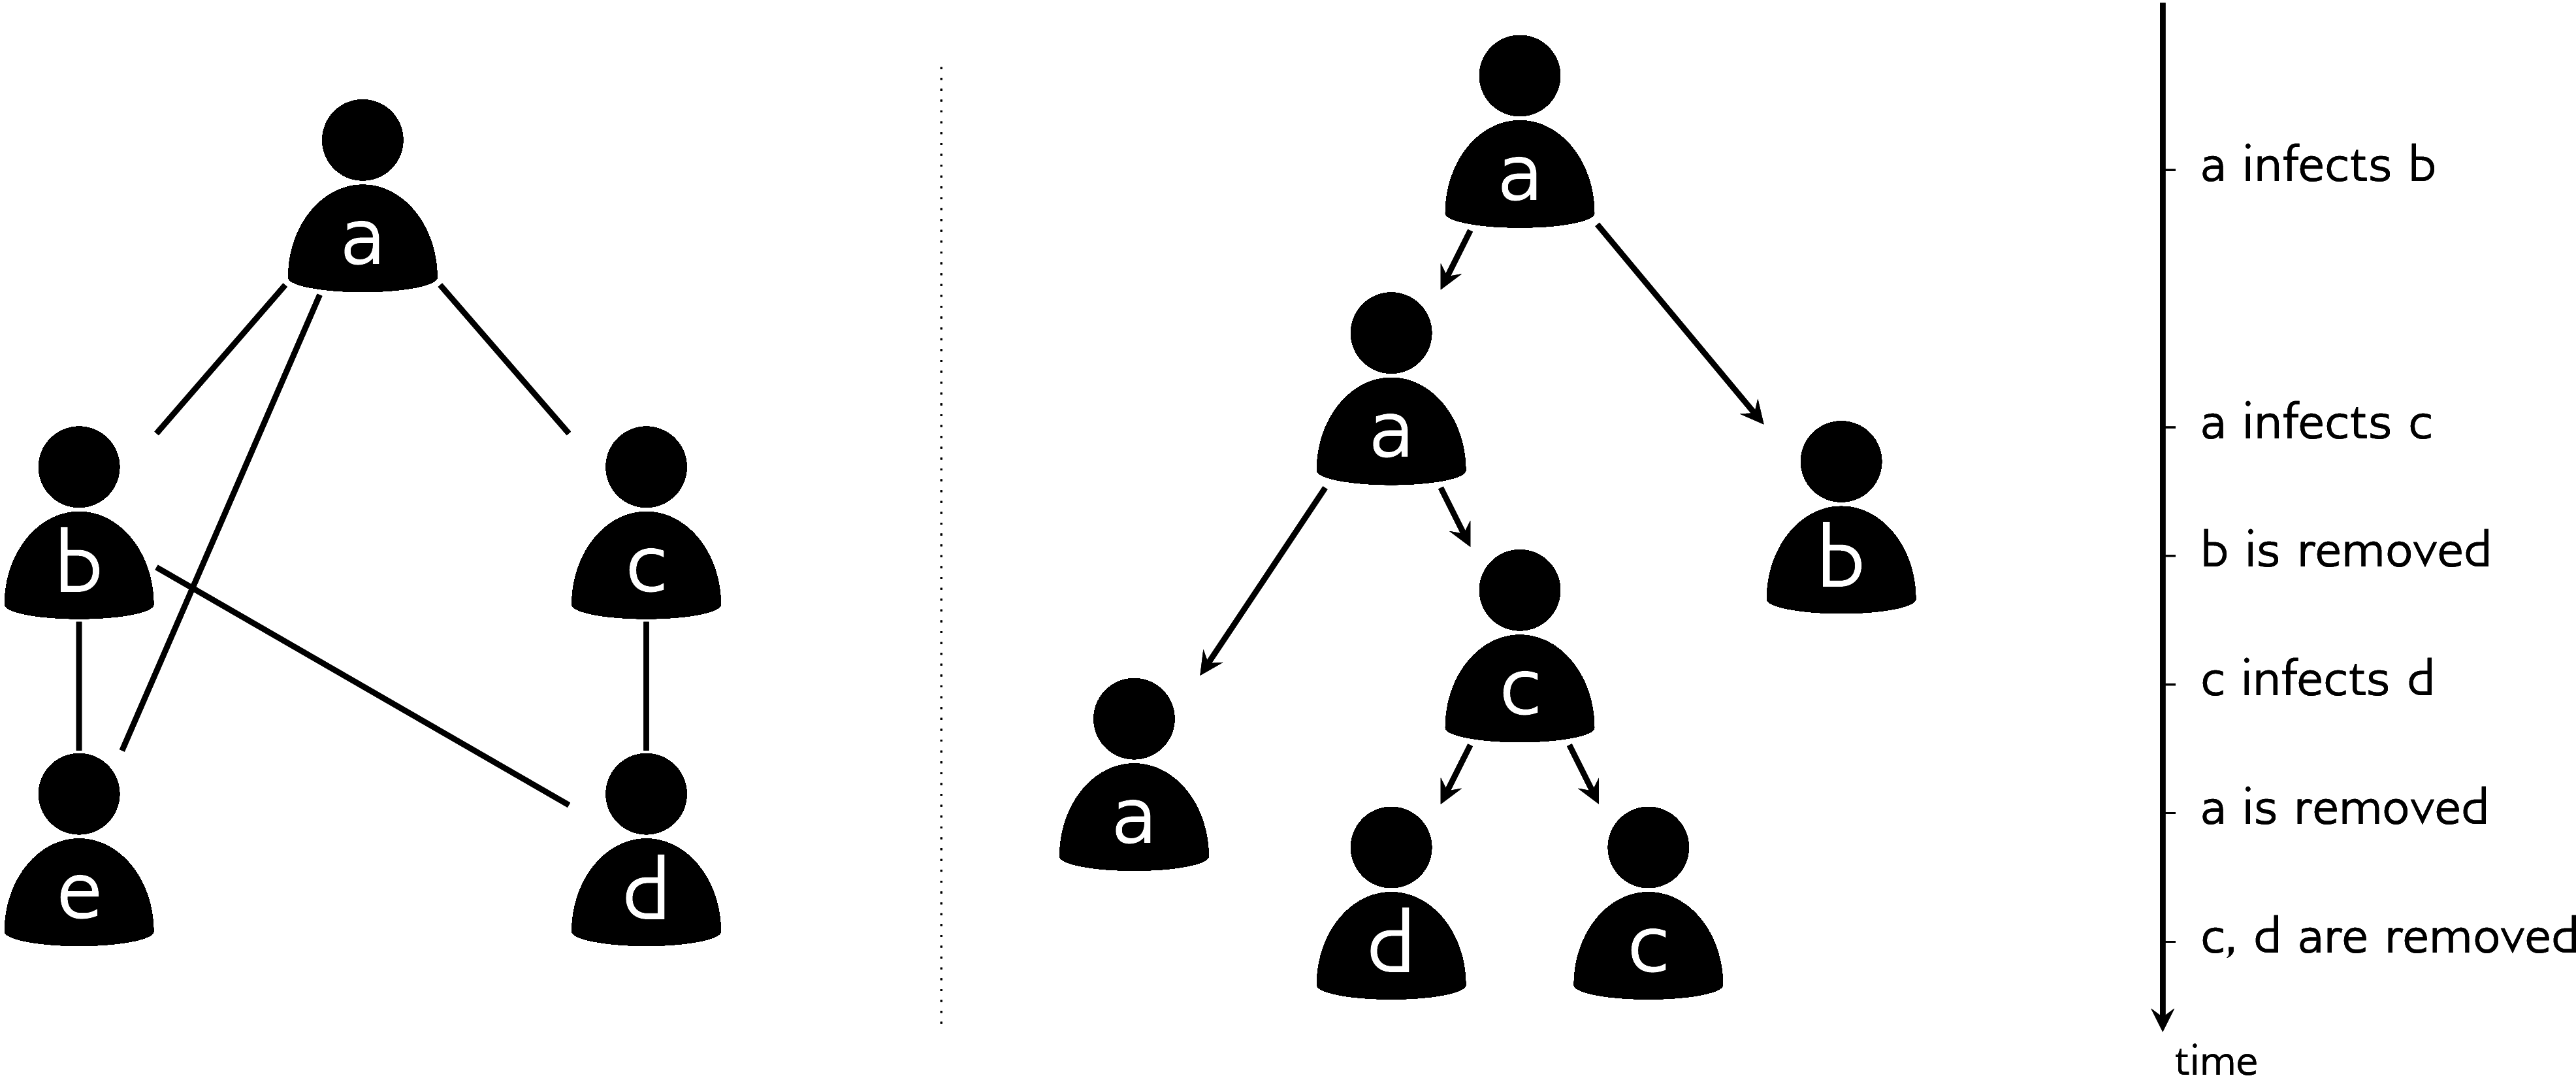
\includegraphics[width=\textwidth]{contactnet.pdf}
    \caption[Illustration of a contact network and transmission tree]{
      Illustration of epidemic spread over a contact network, and the
      corresponding transmission tree. (Left) A contact network with five
      hosts, labelled $a$ through $e$. Thick shaded edges indicate symmetric
      contacts among the hosts. The transmission network is indicated by
      coloured arrows. The epidemic began with node $a$, who transmitted to
      nodes $b$ and $c$. Node $c$ further transmitted to node $d$. Node $e$ was
      not infected. (Right) The transmission tree corresponding to this
      scenario, with a timeline of transmission and removal times.
    }
    \label{fig:contactnet}
\end{figure}

Since transmission trees are essentially a detailed record of an epidemic's
progress, they contain substantial epidemiological information. As a basic
example, the \gls{ltt} plot~\autocite{nee1992tempo}, which plots the number of
lineages in a phylogeny against time, can be used to quantify the incidence of
new infections over the course of an epidemic~\autocite{holmes1995revealing}.
Many more diverse epidemiological parameters have been investigated using
transmission trees, such as the degree of
clustering~\autocite{hughes2009molecular} and the effect of elevated
transmission risk in acute infection~\autocite{volz2012simple}. However, in all
but the most well-studied of epidemics, this is not possible to obtain through
traditional epidemiological methods~\autocite{welch2011statistical}. The time
and effort to conduct detailed interviews and contact tracing of a sufficient
number of infected individuals is usually prohibitive. Even when the resources
for such methods are available, patients may not always recall whom they
contacted and when, especially in the case of airborne transmission.
Consequently, the transmission tree must be estimated using other methods. Most
commonly, this is done by exploiting the relationship between transmission
trees and viral phylogenies~\autocite{volz2013viral}.

\subsection{Relationship between transmission trees and viral phylogenies}

In general, \defn{viral phylogenies} are simply phylogenetic trees relating
virus strains. In phylodynamics, we often consider \defn{inter-host}
phylogenies, which relate one viral genotype from each host in a population.
The crux of \defn{phylodynamics}~\autocite{grenfell2004unifying} is the fact
that the epidemiological processes recorded in transmission trees, and the
evolutionary processes recorded in viral phylogenies, occur on similar time
scales for RNA viruses~\autocite{drummond2003measurably}. As a result, there is
a close relationship between the two types of tree. In particular, the
transmission process is quite similar to \defn{allopatric
speciation}~\autocite{coyne2004speciation}, where genetic divergence follows
the geographic isolation of a sub-population of organisms. Thus, transmission,
which is represented as branching in the transmission tree, causes branching in
the viral phylogeny as well. Similarly, the removal of an individual from the
transmission tree causes the extinction of their viral lineage in the
phylogeny. Due to these relationships, the topology of the viral phylogeny is
often used as a proxy for the topology of the transmission tree. However, there
are several complications and caveats which must be kept in mind when
estimating the transmission tree in this manner.

First are the issues of rooting and time-scaling. Modern likelihood-based
methods of phylogenetic reconstruction~\autocite[\eg][]{price2010fasttree,
stamatakis2014raxml} produce unrooted trees whose branch lengths measure
genetic distance in units of expected substitutions per site. On the other
hand, transmission trees are rooted, and have branches measuring calendar
time~\autocite{pybus2009evolutionary}. It is generally assumed that sampling a
virus from the individual also corresponds to their removal from the
transmission tree, so the positions of the tips in time are fixed. Therefore,
to transform a viral phylogeny into an estimated transmission tree, we must
find a root and an assignment of branch lengths such that the tips are placed
at their proscribed times. In addition, the branch lengths should be chosen
such that the variation in \defn{evolutionary rate}, which is the ratio of a
branch's length in genetic distance to its length in calendar time, is low
across the tree. While there is some variation among hosts, due to
immunological and other factors, we generally expect to observe globally
similar evolutionary rates. Methods for time-scaling a phylogeny include
root-to-tip regression~\autocite{shankarappa1999consistent, korber2000timing,
drummond2003inference}, which we apply in this work, and least-square
dating~\autocite{to2015fast}. Both of these methods can be used to root the
tree, by simply trying all possible root positions and choosing the one which
minimizes a loss function ($1-R^2$, or root-mean-square error, for root-to-tip
regression; sum of squared errors for least-square dating). Alternatively, the
tree may be rooted separately with an outgroup~\autocite{li1988rates} before
time-scaling.

A second, perhaps more insidious problem is the fact that the correspondence
between the topologies of the viral phylogeny and transmission tree is not
necessarily exact. Due to intra-host diversity, the viral strain which is
transmitted may have split from another lineage within the donor long before
the transmission event occurred. Hence, the branching point in the viral
phylogeny may be much earlier than that in the transmission tree. Another
possibility is that one host transmitted to two or more recipients, but the
lineages they each received originated within the donor host in a different
order than that in which the transmissions occurred. In this case, the topology
of the transmission tree and the viral phylogeny will be mismatched. Although
phylodynamics is quite new, these phenomena have been studied in evolutionary
biology for some time. Viral phylogenies are a specific version of a more
general class of trees called \defn{gene trees}, which represent the
evolutionary history of a section of genetic material. Transmission trees, on
the other hand, are highly analogous to \defn{species trees}, whose tips are
species and internal nodes are common ancestors. This analogy derives from the
functional similarity between transmission and allopatric speciation. Hence,
the potential discordance between transmission trees and viral phylogenies is
the similar to that between gene and species trees, which is called
\defn{incomplete lineage sorting}. In practice, this discordance has not proven
an insurmountable problem: for example, \textcite{leitner1996accurate} were
able to accurately recover a known transmission tree using a viral phylogeny.

A final caveat is that the viral phylogeny itself is not known with certainty,
so it must also be estimated from genetic data. Phylogenetic inference is a
complex topic which we will not discuss in detail here (see e.g.
\autocite{nei2000molecular} for a full review). Most modern analyses use
model-based methods, which simultaneously estimate the phylogeny with branch
lengths and the parameters of a model of evolution. Although they usually work
well in practice, the estimated topology can vary based on the model used and,
in the case of Bayesian analysis, the priors.  In addition, intra-host viral
populations are genetically heterogeneous, so choosing a single representative
genotype per host is necessarily imprecise. One can use either the genotype of
a specific virion sampled from the host, or a synthetic genotype, such as a
consensus or reconstructed ancestral sequence.

What we have just discussed is a two-step procedure for estimating the
transmission tree. First, a viral phylogeny is constructed from genetic
sequence data, and then it is rooted and time-scaled into a transmission tree.
This approach is straightforward, frequently used, and has the advantage of
leveraging tried-and-true tools for phylogenetic inference. However, it also
has drawbacks, perhaps the most obvious being the multiplication of errors
produced by the separate steps. One commonly used alternative method is to
directly estimate a time-scaled phylogeny by simultaneously inferring the tree
topology, its root and branch lengths, and the parameters of a \defn{molecular
clock} model. A molecular clock is a hypothesis about the evolutionary rates
along the branches of the tree, such as that they are all equal (a \defn{strict
clock}) or that they are \gls{iid} from a common distribution (a \defn{relaxed
clock}). This inference is usually done in a Bayesian framework using
\gls{MCMC}, so that prior information (including the tip dates) can be included
in the analysis, and the so-called nuisance parameters of the molecular clock
model can be marginalized out. Software packages for performing these analyses
include BEAST~\autocite{bouckaert2014beast} and
MrBayes~\autocite{ronquist2012mrbayes}.

Several other authors have developed methods tailor-made for inferring
transmission trees. \textcite{didelot2014bayesian} develop a Bayesian version
of the two-step approach which allows transmissions to occur anywhere along the
branches of a transmission tree, rather than being constrained to the branching
points in the viral phylogeny. The method requires sampling of every infected
individual, although the authors indicate that it could be extended to relax
this assumption. \textcite{cottam2008integrating} describe a likelihood-based
method which enumerates all transmission trees consistent with an established
phylogeny, assigning each a likelihood based on other epidemiological data. 
This approach is novel in its integration of data from multiple sources,
however because it enumerates a large portion of the tree space, it is unlikely
to scale to larger epidemics. \textcite{ypma2012unravelling} develop a joint 
likelihood function integrating temporal, geographic, and genetic observations, 
and use Bayesian \gls{MCMC} to estimate both the tree and the parameters of the
likelihood function. Their approach can handle missing data and produces high
resolution transmission trees when multiple types of data are available. A
different approach is undertaken by \textcite{jombart2011reconstructing}, who
describe a method to build transmission trees directly from sequence data,
contingent on the common ancestors also being sampled. This makes the method
attractive for slow-evolving pathogens, but less practical for viral outbreaks
where samples from common ancestors are unlikely to be available.

\subsection{Tree shapes}
\label{subsubsec:treeshape}

The aim of viral phylodynamics is to glean some kind of knowledge, about the
epidemic, the virus, or its hosts and their behaviour, by studying a phylogeny,
most often an estimated transmission tree~\autocite{pybus2009evolutionary,
volz2013viral}. What is informative about a phylogeny, beyond the demographic
characteristics of the individuals it relates, is its \defn{shape}. The shape
of a phylogeny has two components: the topology, and the distribution of branch
lengths~\autocite{mooers1997inferring}. Methods of quantifying tree shape fall
into two categories: summary statistics, and pairwise measures.

Summary statistics assign a numeric value to each individual tree. One of the
most widely used is Sackin's index~\autocite{shao1990tree}, which measures the
imbalance or asymmetry in a rooted tree. For the $i$th tip of the tree, we
define $N_i$ to be the number of branches between that tip and the root. The
unnormalized Sackin's index is defined as the sum of all $N_i$. It is called
unnormalized because it does not account for the number of tips in the tree.
Among two trees having the same number of tips, the least-balanced tree will
have the highest Sackin's index. However, among two equally balanced trees, the
larger tree will have a higher Sackin's index. This makes it challenging to
compare balances among trees of different sizes. To correct this,
\textcite{kirkpatrick1993searching} derive the expected value of Sackin' index
under the Yule model~\autocite{yule1925mathematical}. Dividing by this expected
value normalizes Sackin's index, so that it can be used to compare trees of
different sizes.

Rather than assigning numbers to individual trees, pairwise measures associate
a numeric value to each \textit{pair} of trees, indicating how different the
trees are from each other. Distance measures allow us to identify groups of
related phylogenies, for example, local epidemics which are undergoing a
similar pattern of expansion. One such distance measure is the
\gls{nltt}~\autocite{janzen2015approximate}, which compares the
\gls{ltt}~\autocite{nee1992tempo} plots of two trees. Specifically, the two
\gls{ltt} plots are normalized so that they begin at $(0, 0)$ and end at $(1,
1)$, and the difference between the two plots is integrated between 0 and 1. In
the context of infectious diseases, the \gls{ltt} is related to the
prevalence~\autocite{holmes1995revealing}, so large values may indicate that
the trees being compared are the products of different epidemic
trajectories~\autocite{janzen2015approximate}.

Another tree distance measure is the \defn{phylogenetic kernel}, or ``tree
kernel'' developed by \textcite{poon2013mapping}. As opposed to the \gls{nltt},
the tree kernel is maximized when the two trees being compared are the same.
The basis of the tree kernel is the kernel trick originally developed for
\glspl{SVM}~\autocite{burges1998tutorial}. The idea of the kernel trick is to
compare objects by mapping them into a feature space of very high, possibly
even infinite, dimension. The similarity between objects is taken to be their
dot product in the feature space. It is called a ``trick'' because this dot
product is computed using a \defn{kernel function} without explicitly mapping
the objects to the feature space, which would be computationally prohibitive.
In the case of the tree kernel, the feature space is the space of all possible
\defn{subset trees}, which are subtrees that do not necessarily extend all the
way to the tips. The subset-tree kernel was originally developed for comparing
parse trees in natural language processing~\autocite{collins2002new} and did
not incorporate branch length information. The version developed by
\textcite{poon2013mapping} includes a radial basis function to compare the
differences in branch lengths, thus incorporating both the trees' topologies
and their branch lengths in a single similarity score. The tree kernel was
later shown to be highly effective in differentiating trees simulated under a
compartmental model with two risk groups of varying contact
rates~\autocite{poon2015phylodynamic}. In that paper,
\citeauthor{poon2015phylodynamic} used the tree kernel as the distance function
in \gls{ABC} (see \cref{sec:abc}), to fit epidemiological models to observed
trees. This is an example of kernel-ABC~\autocite{nakagome2013kernel}, which
will be discussed further in \cref{sec:abc}.

\subsection{Applications of phylodynamics}
\label{subsec:phyloapp}

Phylodynamic methods have been used to investigate epidemiological parameters
such as transmission rate, recovery rate, and basic reproductive
number~\autocite{pybus2009evolutionary, volz2013viral}. These studies make
inferences about epidemiological processes from the genetic diversity of virus
populations, which is usually represented in the form of a phylogeny. The
majority of these employ a Bayesian \gls{MCMC} approach to infer parameters of
an epidemiological model whose likelihood can be calculated, most often some
variation of the birth-death~\autocite{kendall1948generalized} or
coalescent~\autocite{kingman1982coalescent} models.
\textcite{stadler2011estimating} develop a formula for the likelihood of a
phylogeny with heterochronous tips under the birth-death model, which has been
used to estimate the basic reproductive number of several viral
epidemics~\autocite{stadler2011estimating}. However, the birth-death model is
cannot tell us anything about population structure, as it assumes that every
individual becomes infected at the same rate. \textcite{volz2012complex} writes
down the likelihood of a heterochronous phylogeny under a coalescent model with
arbitrarily complex population dynamics. This opens the door to more complex
inferences about population structure, as the population can be partitioned
into compartments with different transmission and recovery rates, but still
assumes that each compartment is homogeneously mixed. In other words, the
coalescent model can tell us about the \emph{global} structure of a population,
such as whether there exists a high-risk subgroup, but not about the
\emph{local} structure, such as the average number of contacts each individual
has. 

\section{Contact networks}
\label{sec:contactnet}

\subsection{Overview}
\label{subsec:netoverview}

Epidemics spread through populations of hosts through \defn{contacts} between
those hosts. The definition of contact depends on the mode of transmission of
the pathogen in question. For an airborne pathogen like influenza, a contact
may be simple physical proximity, while for \gls{HIV}, contact could be via
unprotected sexual relations or blood-to-blood contact (such as through needle
sharing). A \defn{contact network} is a graphical representation of a host
population and the contacts among its members~\autocite{klovdahl1985social,
morris1993epidemiology, keeling2005networks}. The \defn{nodes} in the network
represent hosts, and \defn{edges} or \defn{links} represent contacts between
them. A contact network is shown in \cref{fig:contactnet} (left). Contact
networks are a particular type of \defn{social
network}~\autocite{moreno1953shall, barnes1954class}, which is a network in
which edges may represent any kind of social or economic relationship. Social
networks are frequently used in the social sciences to study phenomena where
relationships between people or entities are important \autocite[for a review
see][]{wasserman1994social}.

Edges in a contact networks may be \defn{directed}, representing one-way
transmission risk, or \defn{undirected}, representing symmetric transmission
risk. For example, a network for an airborne epidemic would use undirected
edges, because the same physical proximity is required for a host to infect or
to become infected. However, an infection which may be spread through
blood-to-blood contact through transfusions transfusions would use directed
edges, since the donor has no chance of transmitting to the recipient. Directed
edges are also useful when the transmission risk is not equal between the
hosts, such as with HIV transmission, where acting as the receptive partner
carries a higher risk of infection than acting as the insertive partner. In
this case, a contact could be represented by two directed edges, one in each
direction between the two hosts, with the edges annotated by what kind of risk
they imply~\autocite{wasserman1994social}. An undirected contact network is
equivalent to a directed network where each contact is represented by two
symmetric directed edges. The \defn{degree} of a node in the network is how
many contacts it has. In directed networks, we may make the distinction between
\defn{out-degree} and \defn{in-degree}, which count respectively the number
incoming and outgoing edges. The \defn{degree distribution} of a network
denotes the probability that a node has any given number of links. The set of
edges attached to a node are referred to as its \defn{incident} edges.

Epidemiological models most often assume some form of contact homogeneity. The
simplest models, such as the \gls{SIR} model, assume a completely homogeneously
mixed population, where every pair of contacts is equally likely. More
sophisticated models partition the population into groups with different
contact rates between and among each group. However, these models still assume
that every possible contact between a member of group $i$ and a member of group
$j$ is equally likely. This assumption is clearly unrealistic for the majority
of human communities, and can lead to significant errors in predicted epidemic
trajectories when there is substantial heterogeneity
present~\autocite{bansal2007individual, volz2007susceptible}. Contact networks
provide a way to relax this assumption by representing individuals and their
contacts explicitly. It is important to note that, although panmixia is an
unrealistic modelling assumption, it has not proven a substantial hurdle to
epidemic modelling in practice~\autocite{anderson1992infectious}. Using this
assumption, researchers have been able to derive estimates of the transmission
rate and the basic reproductive number of various outbreaks, which have agreed
with values obtained by on-the-ground data collection. Therefore, if one is
interested only in these population-level variables, the additional complexity
of contact network models may not be warranted. Rather, these models are most
useful when we are interested in properties of the network itself, such as
centrality, structural balance, and
transitivity~\autocite{wasserman1994social}.

From a public health perspective, knowledge of contact networks has the
potential to be extremely useful. On a population level, network structure can
dramatically affect the speed and pattern of epidemic
spread~\autocite[\eg][]{barthelemy2005dynamical, volz2008sir}. For example,
epidemics are expected to spread more rapidly in networks having the ``small
world'' property, where the average path length between two nodes in the
network is relatively low~\autocite{watts1998collective}. Some sexually
transmitted infections would not be expected to survive in a homogeneously
mixed population, but their long-term persistence can be explained by contact
heterogeneity~\autocite{anderson1992infectious, pastor2001epidemic}. Hence, the
contact network can provide an idea of what to expect as an epidemic unfolds.
In terms of actionable information, vaccination strategies which would
eradicate an epidemic in a random network might not work if the network is
scale-free~\autocite[][see \cref{subsec:pa}]{keeling2005networks}. On a local
level, contact networks can be informative about the groups or individuals who
are at highest risk of acquiring or transmitting infection, and would therefore
benefit most from public health interventions~\autocite{wang2015targeting,
little2014using}.

Contact networks are a challenging type of data to collect, requiring extensive
epidemiological investigation in the form of contact
tracing~\autocite{morris1993epidemiology, welch2011statistical,
keeling2005networks}. Therefore, it has been necessary to explore less
resource-intensive alternatives which still contain information about
population structure. For instance, it is possible to obtain limited
information about the contact network by individual interviews without contact
tracing. Variables which can be estimated in this fashion are referred to as
\defn{node-level} measures~\autocite{wasserman1994social}. One of the most
well-studied of these is the degree distribution, which can be estimated by
simply asking each person how many contacts they had in some interval of
time~\autocite{liljeros2001web, schneeberger2004scale, colgate1989risk}.

An alternative approach has been the analysis of other networks, which can be
estimated with phylogenetic methods from viral sequence data. Some work focuses
on the \defn{phylogenetic network}, in which two nodes are connected if the
genetic distance between their viral sequences is below some threshold.
Primarily, this work has focused on the detection of \defn{phylogenetic
clusters}, which are groups of individuals whose viral sequences are
significantly more similar to each other's than to the general population's.
The phylogenetic network is informative about ``hotspots'' of transmission and
can be used to identify demographic groups to whom targeted interventions are
likely to have the greatest effect~\autocite{poon2014impact}.  However, this
network may show little to no agreement with a contact data obtained through
epidemiological methods~\autocite{yirrell1998molecular, resik2007limitations,
robinson2013dynamics}, and therefore may be a poor proxy for the contact
network. Other studies~\autocite{brown2011transmission} have investigated the
\defn{transmission network}, which is the subgraph of the contact network
consisting of infected nodes and the edges which led to their
infections~\autocite{welch2011statistical} (\cref{fig:contactnet}, left). It is
possible to estimate the transmission network phylogenetically, although the
methods required for doing so are more sophisticated than for estimating the
phylogenetic network~\autocite{brown2011transmission}. These studies again
mostly focusing on clustering, and also on degree distributions.

Other statistical methods have been developed to infer contact network
parameters strictly from the timeline of an epidemic, using neither genetic
data nor reported contacts. \textcite{britton2002bayesian} developed a Bayesian
method to infer the $p$ parameter of an \gls{ER} network, along with the
transmission and removal rate parameters of the \gls{SI} model, using observed
infection and optionally removal times. However, it was designed for only a
small number of observations, and was unable to estimate $p$ independently from
the transmission rate.  \textcite{groendyke2011bayesian} significantly updated
and extended the methodology of \citeauthor{britton2002bayesian}, and applied
it to a measles outbreak affecting 188 individuals. They were able to obtain a
much more informative estimate of $p$, although this data set included both
symptom onset and recovery times for all individuals, and was unusual in that
the entire contact network was presumed to be infected. \textcite{volz2008sir}
developed differential equations describing the dynamics of the \gls{SIR} model
on a wide variety of random networks defined by their degree distributions.
Although the topic of estimation was not addressed in the original paper,
\citeauthor{volz2008sir}'s method could in principle be used to fit such models
to observed epidemic trajectories, similar to what is done with the ordinary
\gls{SIR} model. \textcite{volz2007susceptible} later extended the method to
dynamic contact networks and applied it to a sexual network relating 99
individuals investigated during a syphilis outbreak.

\subsection{Scale-free networks and preferential attachment}
\label{subsec:pa}

A \defn{scale-free} network is one whose degree distribution follows a power
law, meaning that the number of nodes in the network with degree $k$ is
proportional to $k^{-\gamma}$ for some constant
$\gamma$~\autocite{barabasi1999emergence}. Scale-free networks are
characterized by a large number of nodes of low degree, with relatively few
``hub'' nodes of very high degree. Epidemiological surveys have indicated that
human sexual networks tend to be scale-free~\autocite{liljeros2001web,
schneeberger2004scale, colgate1989risk}. Interestingly, many other types of
network, including computer networks, biological neural networks, metabolic
networks~\autocite{jeong2000large}, and academic co-author networks, also have
the scale-free property.

Several properties of scale-free networks are relevant in epidemiology.  The
high-degree hub nodes are known as
\defn{superspreaders}~\autocite{kemper1980identification}, which have been
postulated to contribute in varying degree to the spread of diseases such as
\gls{HIV}~\autocite{stadler2013uncovering} and
\gls{SARS}~\autocite{shen2004superspreading}. Scale-free networks have no
epidemic threshold~\autocite{pastor2001epidemic}, meaning that diseases with
arbitrarily low transmissibility can persist at low levels indefinitely. This
is in contrast with homogeneously mixed populations, in which transmissibility
below the epidemic threshold would result in exponential decay in the number of
infected individuals and eventual extinction of the pathogen (Anderson \& May,
I think). 

One mechanism which has been shown to lead to scale-free networks is
\defn{preferential attachment}~\autocite{simon1955class, barabasi1999emergence}.
Under this process, networks are formed by starting with a small number $m_0$
of nodes. New nodes are added one at a time until there are a total of $N$ in
the network. Each time a new node is added, $m \geq 1$ edges are added from it
to other nodes in the graph. In the original
formulation~\autocite{barabasi1999emergence}, the partners of the new node are
chosen with probability linearly proportional to their degree. However,
\citeauthor{barabasi1999emergence} suggest extending the model such that the
probability of choosing a partner of degree $d$ is proportional to $d^\alpha$
for some constant $\alpha$, and we use this extension here.

There has been some contention of the idea that contact networks are
scale-free. \textcite{handcock2004likelihood} fit several stochastic models of
partner formation to empirical degree distributions derived from population
surveys of sexual behaviour. They found that a negative binomial distribution,
rather than a power law, was the best fit to five out of six datasets, although
the difference in goodness of fit was extremely small in four out of these
five. \textcite{bansal2007individual} found that an exponential distribution,
rather than a power law, was the best fit to degree distributions of six social
or sexual networks. 

\subsection{Relationship between network structure and transmission trees}

The contact network underlying an epidemic constrains the shape of the
transmission network, which in turn determines the topology of the transmission
tree relating the infected hosts (\cref{fig:contactnet}). The index case who
introduces the epidemic into the network becomes the root of the tree. Each
time a transmission occurs, the lineage corresponding to the donor host in the
tree splits into two, representing the recipient lineage and the continuation
of the donor lineage. \Cref{fig:contactnet} illustrates this correspondence.
It's important to note that, although the order and timing of transmissions
determines the tree topology uniquely, the converse does not hold. That is, for
any given topology, there are in general many transmission networks which would
lead to that topology. In other words, it impossible to distinguish who
transmitted to whom from a transmission tree alone~\autocite{bernard2007hiv}.

A number of studies have made progress in quantifying the relationship between
contact networks and transmission trees. \textcite{o2010contact} simulated
epidemics over networks with four types of degree distribution. They then
estimated the Bayesian skyride~\autocite{minin2008smooth} population size
trajectory in two ways: from the phylogeny, using \gls{MCMC}; and from the
incidence and prevalence trajectories, using the method developed by 
\textcite{volz2009phylodynamics}. They found that the concordance between
the two skyrides, as well as the relationship between the skyride and
prevalence curve, was qualitatively different for each degree distribution.
\textcite{leventhal2012inferring} investigated the relationship between
transmission tree imbalance and several epidemic parameters under four contact
network models, and found that these relationships varied considerably
depending on which model was being considered. \textcite{welch2011network}
simulated transmission trees over networks with varying degrees of community
structure. They found that transmission trees simulated under networks with low
clustering could not generally be distinguished from those simulated under
highly clustered networks, and concluded that contact network clusters do not
affect transmission tree shape. However, more recently,
\textcite{villandre2016assessment} investigated the correspondence between
contact network clusters and transmission tree clusters, and found a moderate
correspondence between the two.

In summary, studies in this group have demonstrated that network structure
profoundly influences tree shape, but have not attempted to quantitatively
infer network parameters from observed trees.

%\section{Approximate Bayesian computation}

%Consider a model $M$, with parameters $\theta$, which we wish to fit to some
%observed data $D$. By ``fit'', we often mean that we want to find particular
%values $\hat{\theta}$ for the parameters which optimize the likelihood of our
%data given those parameters and the model,
%\[
%  \hat{\theta} = \argmax_\theta \Pr(D | M, \theta).
%\]
%This $\hat{\theta}$ is the \defn{maximum likelihood} parameter estimate. Note
%that we are employing a common abuse of notation here, where $\Pr(\cdots)$ is
%being unsed to refer to a probabilty \emph{density} rather than a true
%probability. Alternative to maximum likelihood, we may be interested less in a
%point estimate and more in the posterior distribution of possible values of
%$\theta$ given our data, $\Pr(\theta \mid M, D)$. This will be expanded upon
%below, but for the moment, for illustrative purposes, we restrict our attention
%to the maximum likelihood problem.
%
%If the model we are fitting is sufficiently simple, it may be possible to
%calculate $\hat{\theta}$ directly, using calculus. Most models do not admit
%analytic maximum likeilhood solutions, but if the likelihood any set of
%parameters can be calculated up to a normalizing constant, then
%${\Pr(D \mid M,\theta)}$ can be optimized numerically. A wide range of
%optimization strategies exist, the choice of which to use depending on the
%complexity of the model and whether or not we have access to the gradients of
%the likelihood function with respect to each of the parameters. The majority of
%modelling problems fit into this category, and numerical optimization is
%well-developed and extremely widely used.
%
%However, there are some cases, often when the observed data is of a complex
%type, that explicitly calculating the likelihood of some observed data is
%impossible, even up to a normalizing constant. For example, suppose that we
%want to model a chess player's behaviour. We will set up a simple one-parameter
%model which describes the chess playing process.  The parameter, $a \in [0, 1]$
%indicates the player's eagerness to remove his opponent's pieces from the
%board. We can write down an algorithm for the player's behaviour under such a
%model.
%
%% TODO: don't break this over the page
%
%\begin{algorithmic}
%  \While{the game is not over}
%    \If{I can capture an opponent's piece and $\Uniform(0, 1) < a$}
%      \State{capture the piece}
%    \Else
%      \State{make any other move at random}
%    \EndIf
%  \EndWhile
%\end{algorithmic}
%
%Suppose the observed data are the ending configurations of the board, after the
%player has concluded a game against an opponent with a known value of $a$. The
%model we have designed is very simple, but it is not obvious how to calculate
%the likelihood of a particular ending configuration. Indeed, it seems that the
%only way is to enumerate every possible path the game could have taken, and
%tabulate the ending configurations of each. Clearly, this is infeasible.
%Approximate Bayesian computation was designed for situations like these, where
%exact likelihoods are not available, perhaps due to the model involving an
%algorithm or generative process.



\section{Approximate Bayesian computation}
\label{sec:abc}
\glsreset{ABC}

\subsection{Model fitting}
\label{subsec:mfit}

A \defn{mathematical model} is a formal description of a hypothesized
relationship between some observed data, $\vec{x} = \set{x_1, \ldots, x_n}$,
and outcomes, $\vec{y} = \set{y_1, \ldots, y_n}$. A \defn{parametric} model
defines a family of possible relationships between data and outcomes, indexed
by one or more numeric parameters $\theta$. A \defn{statistical} model
describes the relationship between data and outcomes in terms of probabilities.
Statistical models define, either explicitly or implicitly, the probability of
observing $\vec{y}$ given $\vec{x}$ and, if the model is parametric, $\theta$.
In this context, the observed outcomes are taken to be realizations of random
variables $\vec{Y} = \set{Y_1, \ldots, Y_n}$. Note that it is entirely possible
to have no data $\vec{x}$, only observed outcomes $\vec{y}$. In this case, a
model would describe the process by which $\vec{y}$ is generated.

To illustrate these concepts, consider the well-known linear model. For
clarity, we will restrict our attention to the case of one-dimensional data and
outcomes where each $x_i$ and $y_i$ is a real number. The linear model
postulates that the outcomes are linearly related to the data, modulo some
noise introduced by measurement error, environmental fluctuations, and other
external factors. Formally, $y_i = \beta x_i + \varepsilon_i$, where $\beta$ is
the slope of the linear relationship, and $\varepsilon_i$ is the error
associated with measurement $i$. We can make this model a statistical one by
hypothesizing a distribution for the error terms $\varepsilon_i$; most
commonly, it is assumed that they are normally distributed with variance
$\sigma$. In mathematical terms, $Y_i \sim \beta x_i + \N(0, \sigma^2)$, where
``$\sim$'' means ``is distributed as''. We can see from this formulation that
the model is parametric, with parameters $\beta$ and $\sigma$. Moreover, we can
write down the probability density of observing outcome $y_i$ given the
parameters,
\[
  \Pr(Y_i = y_i \mid \beta, \sigma) = 
  \Pr\left(\N(0, \sigma^2) = y_i - \beta x_i\right).
\]
Note that we have followed the standard statistical abuse of notation and used
``$\Pr$'' to refer to a probability \emph{density}, rather than a probability.
Assuming all the $y_i$ are independent, the probability density of the entire
observed set of outcomes is the product of the probability density of each
individual $y_i$,
\[
  \Pr(\vec{Y} = \vec{y} \mid \beta, \sigma) = 
  \prod_{i=1}^N \Pr(Y_i = y_i \mid \beta, \sigma).
\]

For a general model, the probability density of $\vec{y}$ given the parameters
$\theta$ is also known as the \defn{likelihood}, written $\L$, of $\theta$.
That is, $\L(\theta \mid \vec{y}) = \Pr(\vec{y} \mid \theta)$. The higher the
value of the likelihood, the more likely the observations $\vec{y}$ are under
the model. Thus, the likelihood provides a natural criterion for fitting the
model parameters: we want to pick $\theta$ such that the probability density of
our observed outcomes $\vec{y}$ is as high as possible. The parameters which
optimize the likelihood are known as the \textit{\gls{ML}} estimates, denoted
$\hat{\theta}$. \Gls{ML} estimation is usually performed with numerical
optimization. In the simplest terms, many possible values for $\theta$ are
examined, $\L(\theta \mid \vec{y})$ is calculated for each, and the parameters
which produce the highest value are accepted. Many sophisticated numerical
optimization methods exist, although they may not be guaranteed to find the
true \gls{ML} estimates if the likelihood function is complex. Occasionally, as
in the case of least squares, the \gls{ML} estimates can be found explicitly by
setting the likelihood function's derivatives to zero.

\Gls{ML} estimation makes use only of the data and outcomes to estimate the
model parameters $\theta$. However, it is frequently the case that the
investigator has some additional information or \defn{prior belief} about what
$\theta$ are likely to be. For example, in the linear regression case, the
instrument used to measure the outcomes may have a well-known margin of error,
or the sign of the slope may be obvious from previous experiments. The Bayesian
approach to model fitting makes use of this information by codifying the
investigator's beliefs as a \defn{prior distribution} on the parameters,
denoted $\Pr(\theta)$. Instead of considering only the likelihood, Bayesian
inference focuses on the product of the likelihood and the prior, $\Pr(\vec{y}
\mid \theta) \Pr(\theta)$. Bayes' theorem tells us that this product is related
to the \textit{posterior distribution} on $\theta$,
\[
  \Pr(\theta \mid \vec{y}) = \frac{\Pr(\vec{y} \mid \theta) \Pr(\theta)}
                                  {\Pr(\vec{y})}.
\]

In principle, $\Pr(\vec{y} \mid \theta) \Pr(\theta)$ can be optimized
numerically just like $\L(\theta \mid \vec{y})$, which would also optimize the
posterior distribution. The resulting optimal parameters are called the
\gls{MAP} estimates. However, from a Bayesian perspective, $\theta$ is not a
fixed quantity to be estimated, but rather a random variable with an associated
distribution (the posterior). Therefore, the \gls{MAP} estimate by itself is of
limited value without associated statistics about the posterior distribution,
such as the mean or credible intervals. Unfortunately, to calculate such
statistics, it is necessary to evaluate the normalizing constant
$\Pr(\vec{y})$, which is almost always an intractable integral.

A popular method for circumventing the normalizing constant is the use of
\gls{MCMC} to obtain a sample from the posterior distribution. \Gls{MCMC} works
by defining a Markov chain whose states are indexed by possible model
parameters. The transition probability from state $\theta_1$ to state
$\theta_2$ is taken to be
\[
  \max\left(1, \frac{\Pr(\vec{y} \mid \theta_2) \Pr(\theta_2) q(\theta_2, \theta_1)}
                    {\Pr(\vec{y} \mid \theta_1) \Pr(\theta_2) q(\theta_1, \theta_2)} \right),
\]
where $q(\theta, \theta')$ is a symmetric \defn{proposal distribution} used in
the algorithm to generate the chain. The stationary distribution of this Markov
chain is equal to the posterior distribution on $\theta$. Therefore, if a long
enough random walk is performed on the chain, the distribution of states
visited will be a Monte Carlo approximation of $\Pr(\theta \mid \vec{y})$, from
which we can calculate statistics of interest. Actually performing this random
walk is straightforward and is accomplished via the Metropolis-Hastings
algorithm (\cref{alg:mh}).

\begin{algorithm}
  \label{alg:mh}
  \caption{Metropolis-Hastings algorithm for Markov chain Monte Carlo.}
  \begin{algorithmic}
    \State Draw $\theta$ according to $\Pr(\theta)$
    \Loop
      \State Propose $\theta'$ according to $q(\theta, \theta')$
      \State Accept $\theta \gets \theta'$ with probability
      $\max \left( 1, 
       \dfrac{\Pr(\vec{y} \mid \theta') \Pr(\theta') q(\theta', \theta)}
             {\Pr(\vec{y} \mid \theta\phantom{'}) \Pr(\theta\phantom{'}) q(\theta, \theta')}
       \right)$
    \EndLoop
  \end{algorithmic}
  \label{alg:mh}
\end{algorithm}

\subsection{Overview and motivation for ABC}
\label{subsec:abcoverview}

Most mathematical models are amenable to fitting via one or both of the
approaches, \gls{ML} or Bayesian inference, discussed above. However, there are
some, particularly in the domain of population genetics, for which calculation
of either the likelihood or the product of the likelihood and the prior may be
infeasible. For example, one or both of these quantities may be expressible
only as an intractable integral. \Gls{ABC} is designed for such cases, where
standard likelihood-based techniques for model fitting cannot be applied. Such
models are particularly prevalent in population
genetics~\autocite{beaumont2002approximate, beaumont2010approximate}. We will
begin this subsection by describing \gls{ABC} in general terms. Then, we will
use linear regression as a toy problem to demonstrate how \gls{ABC} could be
applied. Finally, we will give an example of a model which is impractical to
fit using likelihood-based methods, and show how its parameters were estimated
using \gls{ABC}.

Ordinarily, Bayesian inference targets the posterior distribution.

%traditional likelihood criterion
%for model ``goodness'' with one based on simulated data generated by the model.
%Good models should be able to simulate data which closely resemble reality. In
%\gls{ABC}, we are no longer interested in the posterior distribution, but
%rather in the distribution of model parameters which produce data sufficiently
%``close'' to the real data. To formalize this, let $d(\cdot, \cdot)$ be a
%distance function on datasets, and $\varepsilon$ be a tolerance level. 

Of course, linear models can be fit more easily using likelihood-based methods, 
since the likelihood $\L(\theta \mid \vec{y})$ can be easily calculated (see
\cref{subsec:fit}). One model where this is not the case is Kingman's
coalescent~\autocite{kingman1982coalescent}. 

As an example of such a model, we will review the first practical application
of \gls{ABC} by \textcite{tavare1997inferring}. The aim of the investigation
was to calculate the posterior distribution on the coalescence time $t$ of some
observed sequences $D$ under the coalescent model
\autocite{kingman1982coalescent} with the infinite-sites assumption
\autocite{watterson1975number}. Their estimation method relied on two key
observations. First, the number $k$ of \defn{segregating sites} in the data is
informative about the coalescence time while being much easier to work with
than the data itself. A segregating site is a position which is polymorphic in
the observed sequences. Using this observation, the authors replaced their
posterior distribution of interest, $\Pr(t \mid D)$, by
\[
  \Pr(t \mid k) \propto \Pr(t) \Pr(k \mid t),
\]
where again we abuse $\Pr$ to refer to a probability density. Second,
the authors observed that the expected number of segregating sites depends on
the total branch length $l$ of the tree, rather than its height. This enabled
them to write an alternative expression for the product of the likelihood and
prior in terms of $l$,
\[
  \Pr(t) \Pr(k \mid t) = \int_0^\infty \Pr(t, l) \Pr(k \mid l) \d l.
\]
While this integral may be difficult to evaluate analytically, the power of
this formulation is the fact that it is straightforward to \emph{simulate}
values of $t$ and $l$ according to $\Pr(t, l)$, their joint probability under
the coalescent model. One simply runs the (stochastic) coalescent process and
observing the values $\hat{t}$ and $\hat{l}$ which result. It is
straightforward to calculate $\Pr(k \mid \hat{l})$, the probability
that $k$ segregating sites were observed in a tree with total branch length
$\hat{l}$, using the Poisson distribution. Hence if $\hat{l}$ and $\hat{t}$,
having been generated according to $\Pr(t, l)$, are sampled with probability
proportional to $\Pr(k \mid \hat{l})$, they represent an unbiased sample from
the above integral. Taking a large number of such samples allowed the authors
to obtain a Monte Carlo estimate of $\Pr(t \mid k)$.

%\Gls{ABC} is a statistical method designed to fit complex models, which cannot
%be fit using more conventional methods, to observed
%data~\autocite{marin2012approximate, sunnaker2013approximate,
%beaumont2010approximate}. We shall make this precise below, but to fully
%describe and motivate \gls{ABC}, it is necessary to first explain exactly what
%we mean by ``fitting'' a model. We will illustrate this concept with one of the
%simplest and most ubiquitous models: linear regression.
%
%An approximate Bayesian computation approach to least-squares regression might
%be as follows. We will need to make an additional assumption: that the errors
%$\varepsilon_i$ are normally distributed. That is, our linear model is now of
%the form
%\[
%  y_i = bx_i + \N(0, \sigma),
%\]
%where $\N(0, \sigma)$ indicates a normal distribution with mean zero and
%variance $\sigma$. We do not know $\sigma$ in advance, so this is another
%parameter we will need to estimate. There is nothing special about normal
%distributions - we could have chosen any other distribution we deemed
%appropriate. 
%

\subsection{Algorithms for ABC}
\label{subsubsec:abcalg}

\Gls{ABC} does not refer to a particular procedure for model fitting. Rather,
\gls{ABC} refers to the general strategy of choosing model parameters based on
the resulting model's propensity to generate data resembling the real data.
There are three main classes of \gls{ABC} algorithm which have been developed
so far: rejection, \gls{MCMC}, and \gls{SMC}.

All of these approaches require some common elements. First, as with all
Bayesian methods, we are required to specify a \defn{prior distribution},
denoted $\pi$, on the parameter space. The prior specifies what we already know
or believe about the model parameters. Second, in order to compare simulated to
observed data, we need to be able to summarize a data set in a numerical
format. This is accomplished by a function, denoted $\eta$, which computes a
vector of hopefully informative summary statistics on a data set. Third, we
need a distance function $\rho$ which tells us how similar two data sets are to
each other, based on their summary statistics.

Continuing with the linear model example, we need to specify a prior $\pi(a, b,
\sigma)$ on the three parameters. We do not have much certain information about
these parameters except that $\sigma$ has to be at least zero, but it seems
reasonable to assume that extreme relationships are fairly rare, and that
positive and negative correlations are equiprobable. Therefore, we will let
$a$, $b$, and $\sigma$ be independent, $a$ and $b$ be normally distributed,
and $\sigma$ be log-normally distributed. That is,
\[
  \pi(a, b, \sigma) = 
  \begin{cases}
    \Pr[\N(0, 1) = a] \cdot \Pr[\N(0, 1) = b] \cdot \Pr[\N(0, 1) = \log\sigma]
     & \sigma > 0 \\
    0 & \sigma \le 0.
  \end{cases}
\]
For the vector of summary statistics, we will use the mean and variance of the
simulated data,
\[
  \eta(\vec{y}) = \left<\E[\vec{y}], \Var[\vec{y}]\right>.
\]
Finally, for the distance function $\rho$ we take the standard Euclidean
distance.

Rejection ABC is the simplest method, and also the one which was first
proposed~\autocite{rubin1984bayesianly}. Effectively, it comes down to the
approach described in the previous subsection of guessing parameter values
until one is close enough to the truth. More specifically, a possible set of
parameters $\theta$ is drawn from the prior distribution, and a simulated data
set $z$ is generated from the model with those parameters. If the distance
between the simulated data set and the real data, $\rho(\eta(y), \eta(z))$, is
small enough, then we accept $\theta$ as a sample from the posterior. This can
be repeated until as many samples as desired are obtained.

% MCMC
The second method is \gls{ABC}-\gls{MCMC}. This is similar to ordinary Bayesian
\gls{MCMC}, except that a ratio of distances to the observed data replaces the
likelihood ratio. The algorithm begins by sampling a single vector of parameter
values $\theta$ from the prior distribution $\pi(\theta)$. It then proceeds
iteratively: a new parameter vector $\theta^*$ is chosen according to a
proposal distribution $q(\theta^* \mid \theta)$. The proposal distribution $q$
is often taken to be a Gaussian centred at $\theta$. Then $\theta^*$ is
accepted as the new $\theta$ with probability
\[
  \max\left(1, \text{TODO} \right),
\]
or discarded otherwise. This process is iterated until some stopping criterion
is reached, typically a simple limit on the number of steps. After some initial
number of iterations, known as \defn{burn-in}, parameters $\theta$ are
routinely sampled. Since points in parameter space are visited in proportion to
their posterior probability, these samples can be taken to approximate the
posterior distribution on $\theta$, and can be used to calculate point
estimates and confidence intervals.

The most recently developed class of algorithms for ABC is sequential
Monte-Carlo (SMC)~\autocite{sisson2007sequential}. As with the other two
classes, we want to eventually obtain a sample from the posterior distribution
$f(\theta \mid D)$. The idea of SMC is to begin with a sample from a
distribution we know, most often the prior, and approach the posterior smoothly
by progressing through a series of intermediate distributions.

\section{Sequential Monte Carlo}

\Gls{SMC} is a statistical inference method which samples from a sequence of
probability distributions in a fixed order~\autocite{del2006sequential}. This
idea of \defn{sequential sampling} is useful several contexts, but we consider
here its application to model fitting in a Bayesian setting. 

\texttt{TODO: move the basics of model fitting (likelihoods and priors) to here}

Our objective is to obtain samples from, and summary statistics of, the
posterior distribution on the model of interest's parameters. \gls{SMC} can be
applied in this context by defining a sequence of distributions, starting from
the posterior and ending at the prior, which constitute a ``smooth''
trajectory. The main \gls{SMC} algorithm for this problem was developed by
\textcite{del2006sequential}, based on an existing methodology called
\gls{SIS}. \gls{SIS} is also designed to sample from a sequence of
distributions, but rather than all being defined on the same space (such as
model parameters), they are defined on nested spaces of increasing dimension.
Following \textcite{del2006sequential} and other reviews of
\gls{SMC}~\autocite{doucet2001introduction}, we will begin this section by
describing \gls{SIS}, and then turn to the adaptation of the method to the case
when the sequence of distributions are all defined on the same space. Note that
\textcite{del2006sequential} use the variable $\pi$ for the target
distributions, but \textcite{doucet2001introduction} use $\pi$ to indicate the
importance distributions. We follow the former and denote target distributions
by $\pi$ and importance distributions by $\eta$.

\subsection{Sequential importance sampling}

The basis of \gls{SIS} is \gls{IS}, which is a method of estimating summary
statistics of distributions which are known only up to a normalizing constant,
and therefore cannot be sampled from directly. That is, if $\pi$ is such a
distribution and $f$ is any real-valued function, \gls{IS} is concerned with
estimating
\[
  \pi(f) = \int f(x)\pi(x)\d x = \int f(x) \frac{\gamma(x)}{Z} \d x,
\]
where the integral is over the space on which $\pi$ is defined, $\gamma(x)$ is
known, and $Z$ is the unknown normalizing constant, $Z = \int \gamma(x) \d x$.
The posterior distributions of all but the simplest models' parameters fall
into this category. Suppose we have at hand another distribution $\eta$, called
the \defn{importance distribution}, from which we are able to sample. Define
the \defn{importance weight} as the ratio ratio $w(x) = \gamma(x)/\eta(x)$. We
can express the normalizing constant $Z$ in terms of the importance weight and
distribution, $Z = \int w(x) \eta(x) \d x$, and in turn write the original
integral of interest as
\[
  \int f(x) \pi(x) \d x = \frac{\int f(x) \gamma(x) \d x}
                               {\int w(x) \eta(x) \d x}.
\]
If we sample a large number of points from $\eta$, then $\eta(x)$ can be
approximated at each of them by an empirical distribution. Since the remaining
quantities $f$, $\gamma$, and $w$ can all be evaluated pointwise, these are all
the ingredients we need to obtain an estimate of $\pi(f)$. Although this is a
simple and elegant approach, the drawback is that the variance of the estimate
is proportional to the variance of the importance
weights~\autocite{liu2008monte}, which may be quite large if $\eta$ and
$\gamma$ are very different. Therefore, the practical use of \gls{IS} on its
own is limited, since it depends on finding an importance distribution which is
similar to $\pi$, which we usually know very little about \textit{a priory}.

However, an ideal context for the use of \gls{IS} is when we want to sample
from a sequence of nested probability distributions $\pi_1, \ldots, \pi_n$.
By \defn{nested}, we mean that $\pi_{i+1}$ is defined on a space of dimension
$i+1$ and admits $\pi_i$ as a marginal. That is,
\[
  \pi_{i+1}(x_1, \ldots, x_{i+1}) = \pi_i(x_1, \ldots, x_i) f_{i+1}(x_1, \ldots, x_{i+1}),
\]
where $f_{i+1}$ is a function which yields a distribution when multiplied with
$\pi_i$. This situation may seem somewhat contrived, but it arises naturally
when trying to infer the hidden sequence of parameters of a stateful model. For
example, \textcite{doucet2001introduction} discuss the case when $\pi_i$ is the
posterior distribution over the first $i-1$ states of a \gls{HMM}, conditional
on the observed data up to time $i-i$. We assume that either $\pi_1$ is known
explicitly, or we have enough information about it to find an adequate
importance distribution. In the \gls{HMM} example, $\pi_1$ was taken to be the
prior distribution on the starting state.
